\chapter{序論} \label{chap:introduction}

\begin{figure}[htbp]
  \begin{center}
    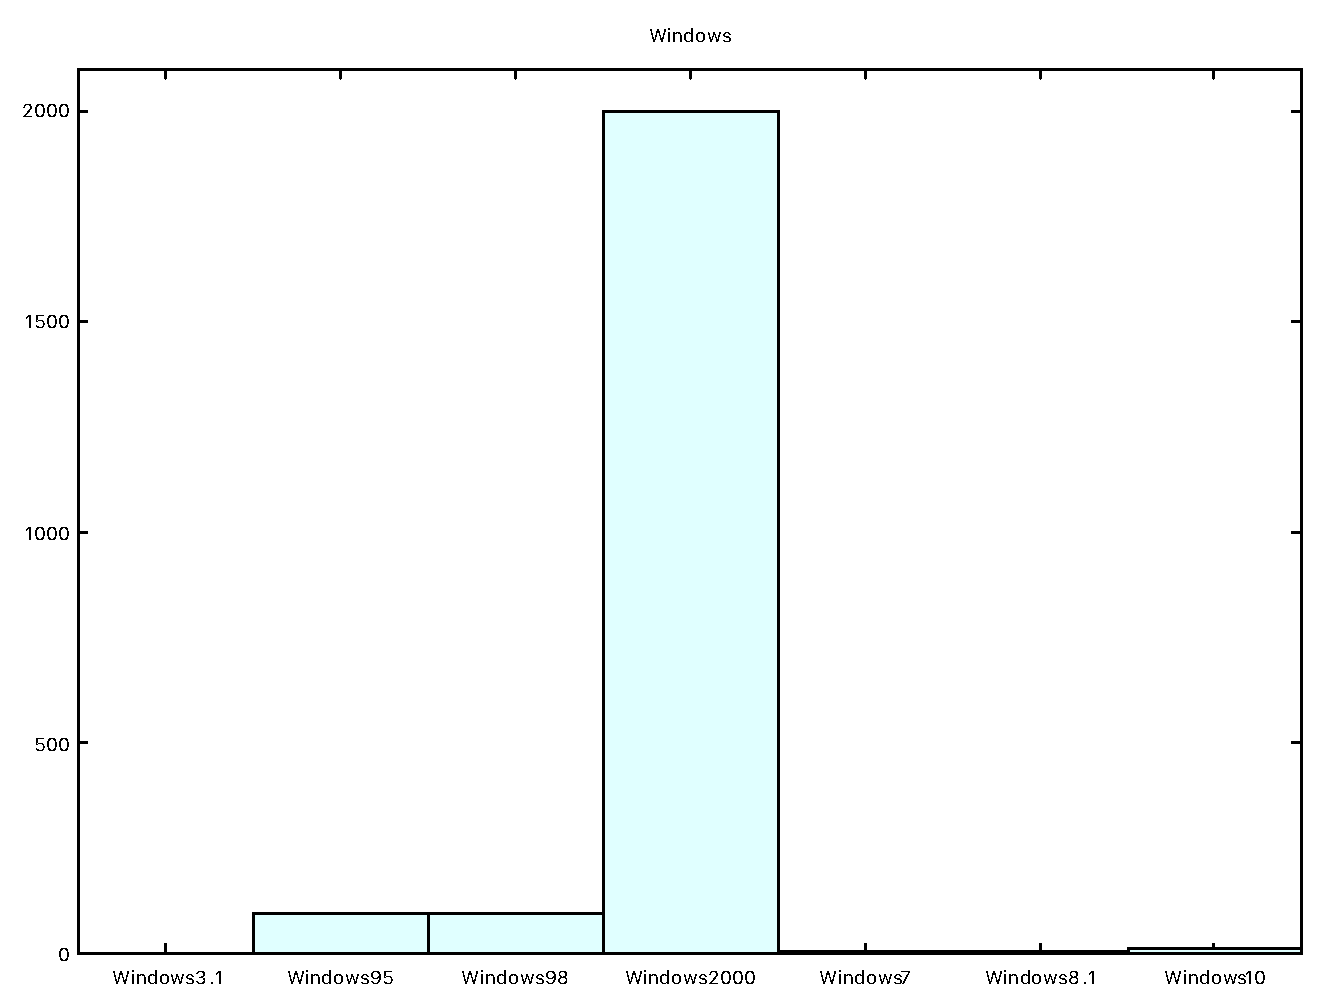
\includegraphics[width=\textwidth]{Windows.pdf}
  \end{center}
  \caption{Windows OS}
  \label{fig:Windows}
\end{figure}

\begin{table}[htbp]
  \begin{center}
    \begin{tabular}{cccc}\toprule
      バージョン & コードネーム & 読み方 & リリース\\ \midrule
      Mac OS X 10.0 & Cheetah & チーター & 2001年3月\\
      Mac OS X 10.1 & Puma & ピューマ & 2001年9月\\
      Mac OS X 10.2 & Jaguar & ジャガー & 2002年8月\\
      Mac OS X 10.3 & Panther & パンサー & 2003年10月\\
      Mac OS X 10.4 & Tiger & タイガー & 2005年4月\\
      Mac OS X 10.5 & Leopard & レパード & 2007年10月\\
      Mac OS X 10.6 & Snow Leopard & スノー レパード & 2009年8月\\
      Mac OS X 10.7 & Lion & ライオン & 2011年7月\\
      OS X 10.8 & Mountain Lion & マウンテン ライオン & 2012年7月\\
      OS X 10.9 & Mavericks & マーベリックス & 2013年10月\\
      OS X 10.10 & Yosemite & ヨセミテ & 2014年10月16日\\
      OS X 10.11 & El Capitan & エル キャピタン & 2015年10月1日\\
      macOS 10.12 & Sierra & シエラ & 2016年9月20日\\
      macOS 10.13 & High Sierra & ハイ シエラ & 2017年9月25日\\
      macOS 10.14 & Mojave & モハベ & 2018年9月25日\\
      macOS 10.15 & Catalina & キャタリナ & 2019年10月7日\\
      macOS 11.0 & Big Sur & ビッグサー & 2020年11月12日\\ \bottomrule
    \end{tabular}
  \end{center}
  \caption{Mac OS}
  \label{tb:Mac}
\end{table}

第\ref{chap:introduction}章しかないけど許して.図\ref{fig:Windows}.表\ref{tb:Mac}.\par
Tensor Renormalization Group\cite{PhysRevLett.99.120601}.